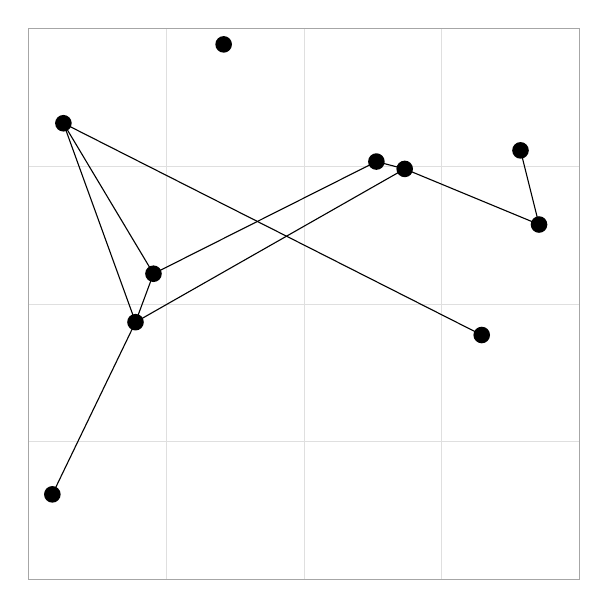
\begin{tikzpicture}[x=1.75cm, y=1.75cm]
% Generated by scripts/generate_sirg.py: seed=42, vertices=10, process=poisson(intensity=0.5), line width=0.4pt, opacity=1
% Ambient window
\draw[step=1, very thin, gray!25]
    (-2,-2) grid (2,2);
\draw[thin, gray!70]
    (-2,-2) rectangle (2,2);

% Vertices
\coordinate (v0) at (1.70706,0.57546048);
\coordinate (v1) at (1.2910465,-0.2263432);
\coordinate (v2) at (-1.0910451,0.21833915);
\coordinate (v3) at (-1.744731,1.3105247);
\coordinate (v4) at (0.5266576,1.032351);
\coordinate (v5) at (-0.58189613,1.8827921);
\coordinate (v6) at (1.5724845,1.113534);
\coordinate (v7) at (-1.2214452,-0.13311599);
\coordinate (v8) at (-1.8247849,-1.382842);
\coordinate (v9) at (0.73219581,0.97904862);

% Edges
\draw[line width=0.4pt, opacity=1] (v0) -- (v6);
\draw[line width=0.4pt, opacity=1] (v0) -- (v9);
\draw[line width=0.4pt, opacity=1] (v1) -- (v3);
\draw[line width=0.4pt, opacity=1] (v2) -- (v3);
\draw[line width=0.4pt, opacity=1] (v2) -- (v4);
\draw[line width=0.4pt, opacity=1] (v2) -- (v7);
\draw[line width=0.4pt, opacity=1] (v3) -- (v7);
\draw[line width=0.4pt, opacity=1] (v4) -- (v9);
\draw[line width=0.4pt, opacity=1] (v7) -- (v8);
\draw[line width=0.4pt, opacity=1] (v7) -- (v9);

% Vertices
\foreach \v in {v0,v1,v2,v3,v4,v5,v6,v7,v8,v9} {
    \fill (\v) circle (3pt);
}
\end{tikzpicture}
